%This is a Tex Version of Math 304 Homework Template
%
\documentclass{amsart}
\setlength{\textheight}{9in}
\setlength{\topmargin}{-0.25in}
\setlength{\textwidth}{7in}
\setlength{\evensidemargin}{-0.25in}
\setlength{\oddsidemargin}{-0.25in}
\usepackage{amsfonts}
\usepackage[utf8]{inputenc}
\usepackage[T1]{fontenc}
\usepackage{graphicx} 
\usepackage[export]{adjustbox}
% needed to include these graphics
%\graphicspath{{./Pictures/}}      % only in case you want to keep the pictures in a separate
                                  % subdirectory; also see the appropriate line below
\usepackage{caption}
\usepackage{subcaption}
\usepackage{float}
\usepackage{framed}
\newcounter{temp}
\theoremstyle{definition}
\newtheorem{Thm}{Theorem}
\newtheorem{Prob}{Problem}
\newtheorem*{Def}{Definition}
\newtheorem*{Ans}{Answer}
\newcommand{\dis}{\displaystyle}
\newcommand{\dlim}{\dis\lim}
\newcommand{\dsum}{\dis\sum}
\newcommand{\dint}{\dis\int}
\newcommand{\ddint}{\dint\!\!\dint}
\newcommand{\dddint}{\dint\!\!\dint\!\!\dint}
\newcommand{\dt}{\text{d}t}
\newcommand{\dA}{\text{d}A}
\newcommand{\dV}{\text{d}V}
\newcommand{\dx}{\text{d}x}
\newcommand{\dy}{\text{d}y}
\newcommand{\dz}{\text{d}z}
\newcommand{\dw}{\text{d}w}
\newcommand{\du}{\text{d}u}
\newcommand{\dv}{\text{d}v}
\newcommand{\ds}{\text{d}s}
\newcommand{\dr}{\text{d}r}
\newcommand{\dth}{\text{d}\theta}
\newcommand{\bbR}{\mathbb{R}}
\newcommand{\bbN}{\mathbb{N}}
\newcommand{\bbQ}{\mathbb{Q}}
\newcommand{\bbZ}{\mathbb{Z}}
\newcommand{\bbC}{\mathbb{C}}
\newcommand{\dd}[2]{\dfrac{\text{d}#1}{\text{d}#2}}
\newcommand{\dydx}{\dfrac{\text{d}y}{\text{d}x}}
\renewcommand{\labelenumi}{{\normalfont \arabic{enumi}.}}
\renewcommand{\labelenumii}{{\normalfont \alph{enumii}.}}
\renewcommand{\labelenumiii}{{\normalfont \roman{enumiii}.}}
\font \bggbf cmbx18 scaled \magstep2
\font \bgbf cmbx10 scaled \magstep2
\usepackage{fancyhdr}
\usepackage{lipsum}
% Clear the header and footer
\fancyhead{}
\fancyfoot{}
% Set the right side of the footer to be the page number
\rfoot{\thepage}
\fancyhf{}
\pagestyle{fancy}
\begin{document}
\LARGE{NE806: Neutronics}
 
\large
Homework \# 1 due Thurs. September 20, 2018
 
Solutions by: John Boyington
\newline
\bigskip
 
 
\textbf{Problem 1:} For light nuclei, elastic scattering is isotropic in the COM frame; this is called s-wave scattering.For heavier nuclei and t higher neutron energies, elastic scattering is not truly isotropic in the COM frame; this is called p-wave scattering. Assuming rotational invariance, we can write
$f(\omega_c, \psi) = \frac{1}{2\pi} f_\omega (\omega_c)$ \newline
(a) (5 points) Write the PDF $f_\omega(\omega_c)$ for s-wave scattering. \newline
(b) (5 points) Assume the joint PDF for a given p-wave scattering case is given by
\begin{equation*}
    f(\omega_c, \psi) = \frac{K}{2\pi} [1+\omega_c], -1 \leq \omega_c \leq 1, \qquad 0 \leq \psi \leq 2\pi
\end{equation*}
what must the value of K be? \newline
(c) (5 points) For part (b), plot the PDFs for $\omega_c$ and $\psi$. \newline
(d) (10 points) For s-wave scattering, the PDF of part (b), what is the PDF for the final neutron energy E' for neutrons of initial energy E? \newline

\textbf{Solution}

(a)
The following equation represents the PDF for s-wave scattering:\\

$$ \boxed{f_\omega(\omega_c) = \frac{1}{2}, -1 \le \omega_c \le 1} $$ \\

(b)
$$ f(\omega_c, \psi) = \frac{\kappa}{2\pi} [1 + \omega_c] $$

Any pdf, when integrated over its domain should equal 1.

$$ 1 = \frac{\kappa}{2\pi} \int^{2\pi}_0 d\psi \int^1_{-1} (1 + \omega_c)d\omega_c $$
$$ 1 = \kappa [\omega_c + \frac{1}{2}\omega_c^2] |^1_{-1} $$
$$ 1 = 2\kappa $$

Leading us to the conclusion: \\
$$ \boxed{\kappa = \frac{1}{2}} $$

(c)

The PDFs for $\psi$ and $\omega_c$ are given in the following figures:\\

\begin{figure}[h!]
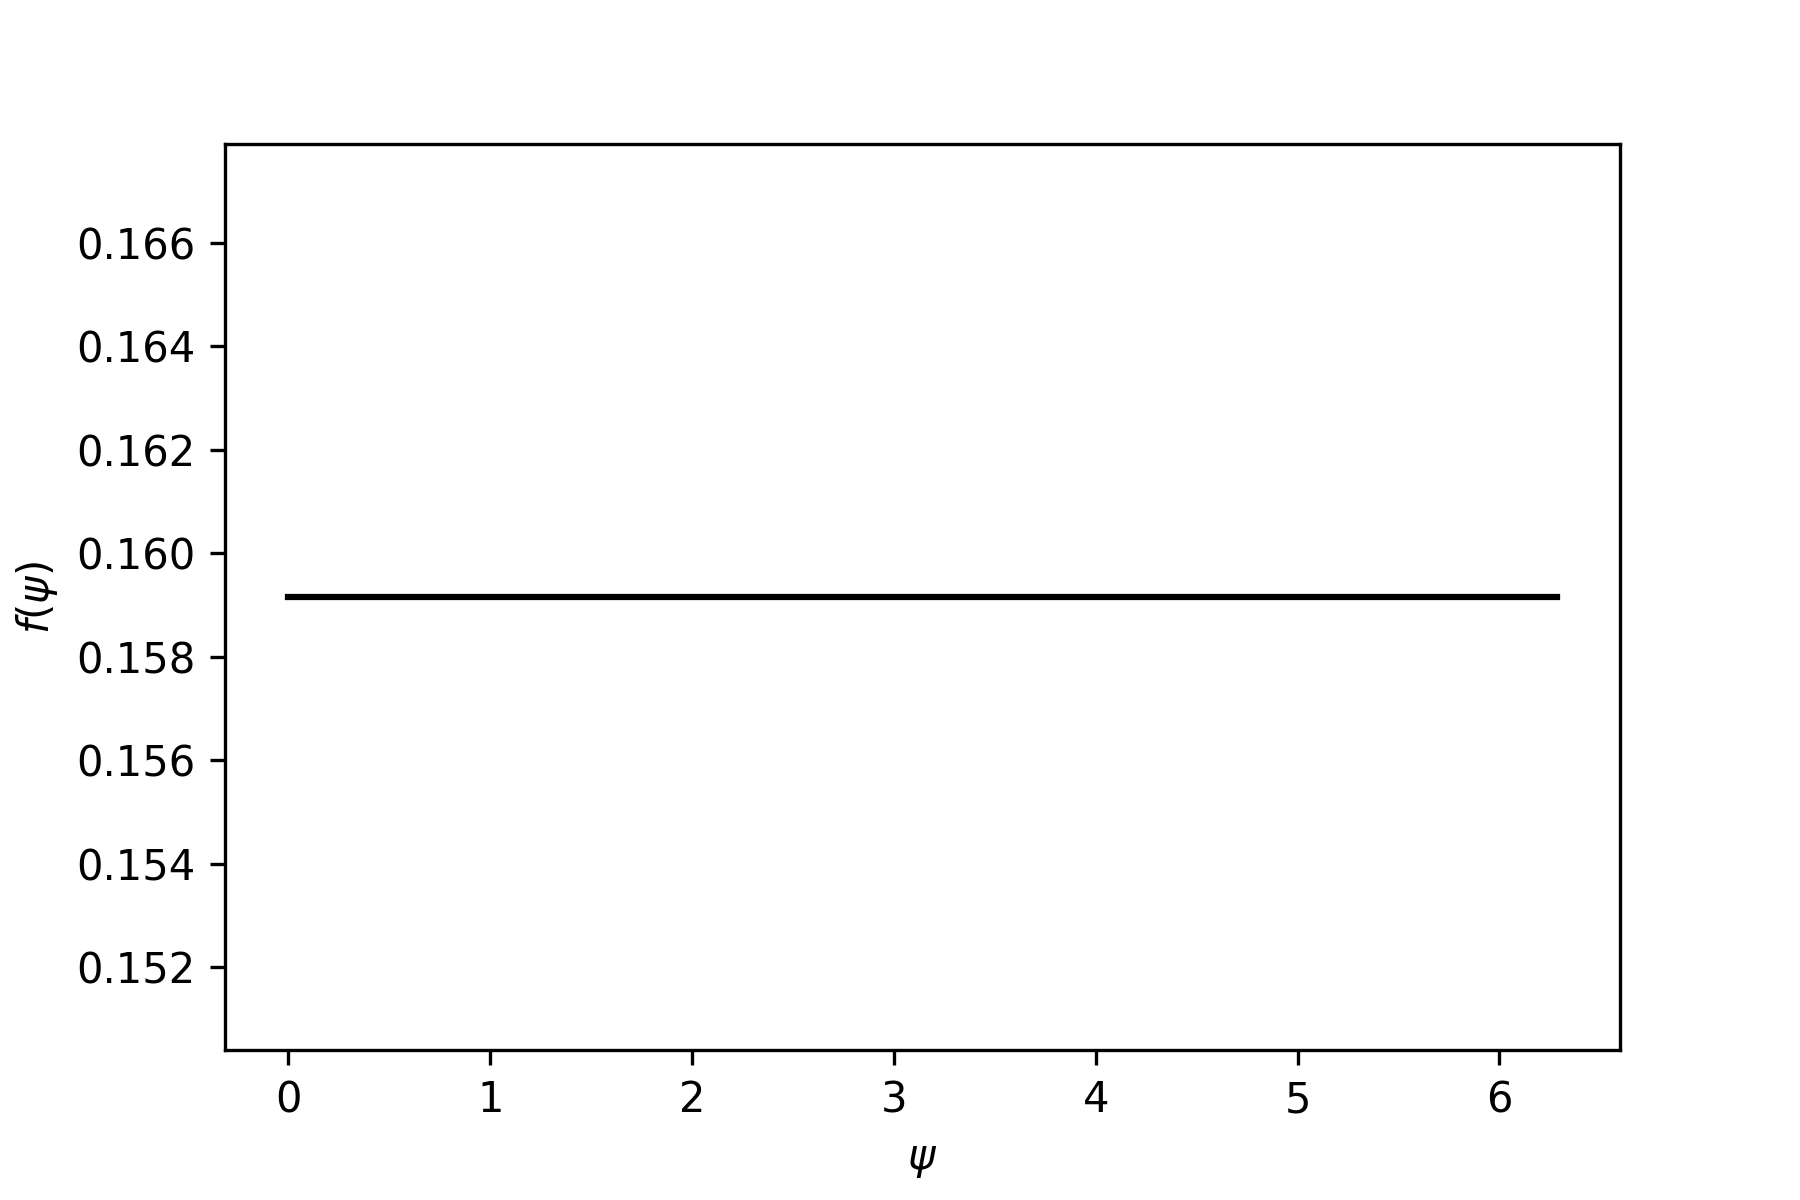
\includegraphics[width=0.6\linewidth]{p1_1.png}
\end{figure}


\begin{figure}[h!]
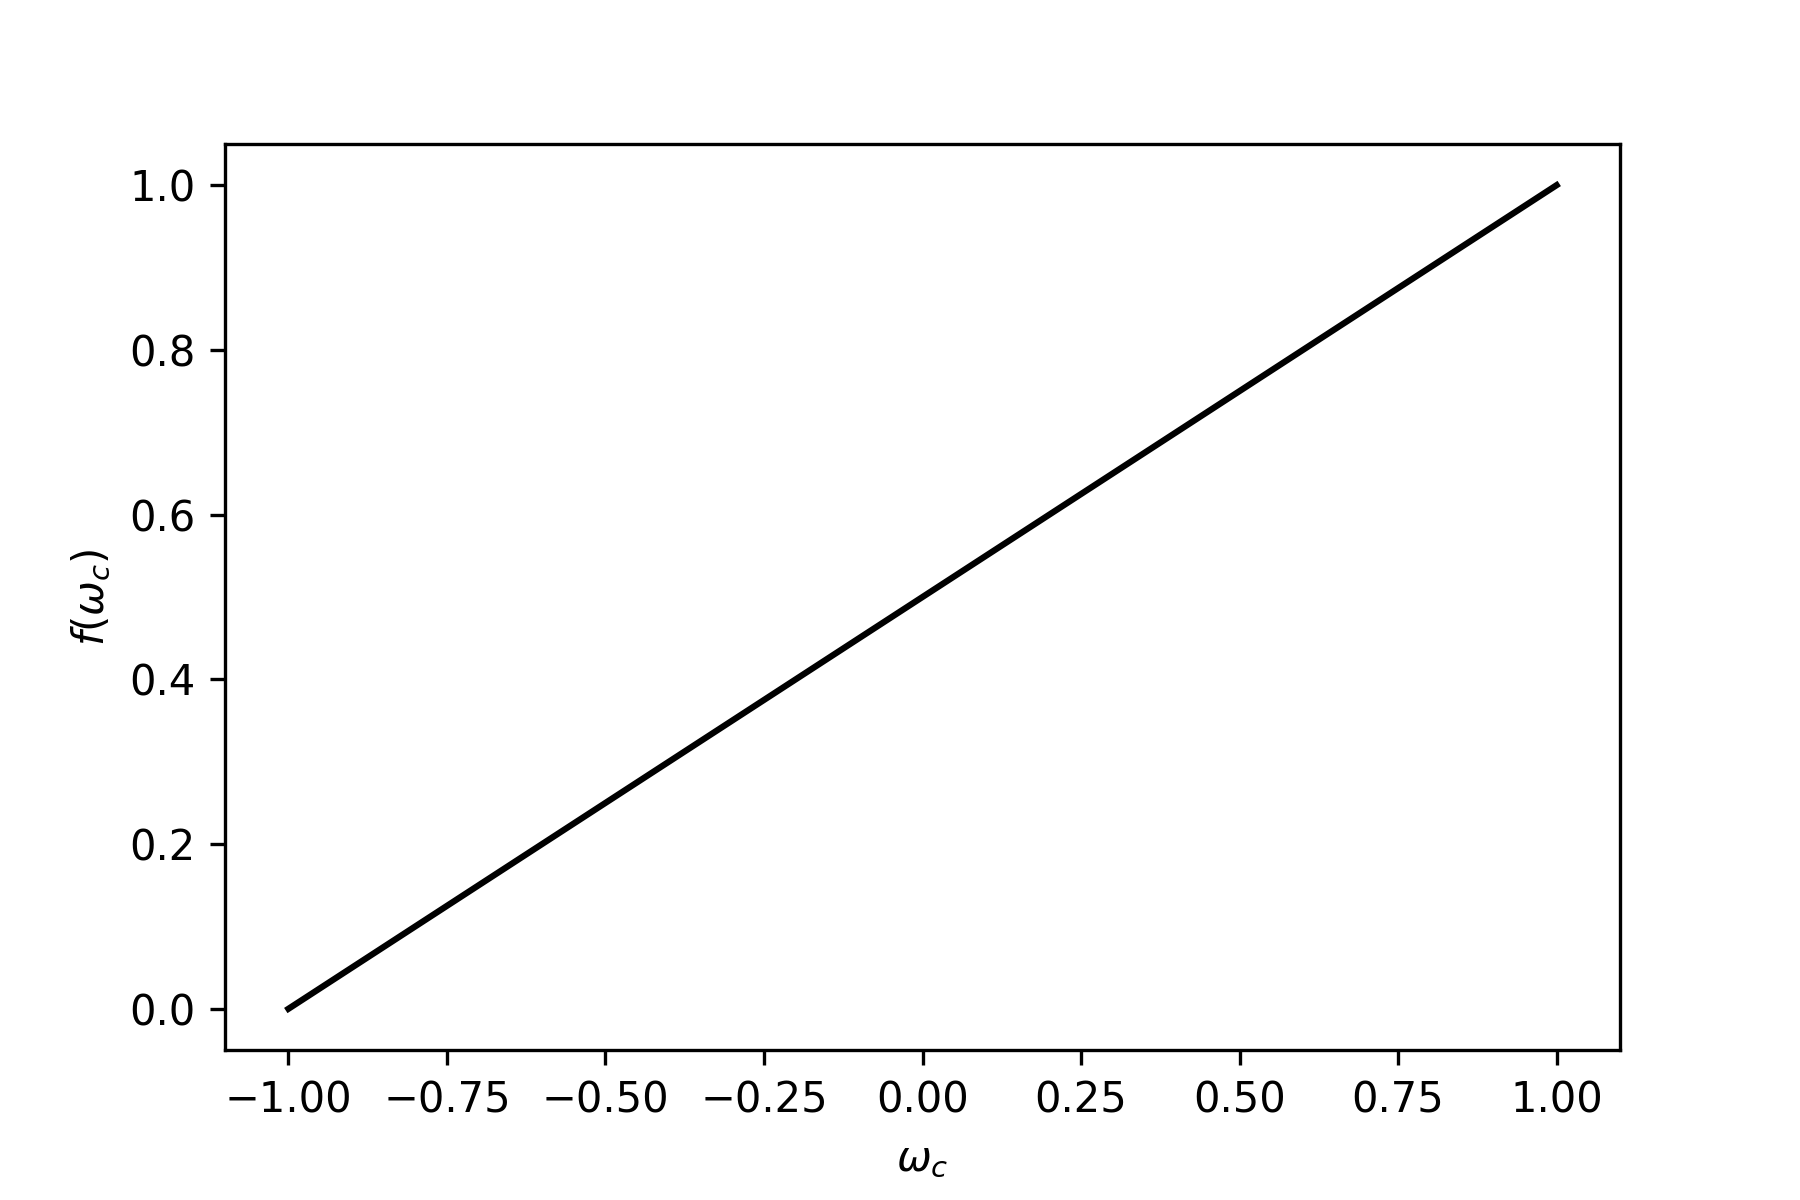
\includegraphics[width=0.6\linewidth]{p1_2.png}
\end{figure}

These were found by integrating the other variable out.

\vspace{0.2\textheight}
(d)

Knowing:
$$ f(\omega_c) = \frac{1}{2} [1 + \omega_c] $$

and using the following relationship:

$$ \frac{E'}{E} = \frac{(1 + \alpha) + (1 - \alpha) \omega_c}{2} $$

we can solve for $\omega_c$.

$$ \omega_c = \frac{2\frac{E'}{E} - (1 + \alpha)}{(1 - \alpha)} $$

where $E'$ is bounded in the following way: $\alpha E \le E' \le E$

Substituting into the equation for $f(\omega_c)$, we get

\boxed{ P(E \rightarrow E') = \frac{1}{2} [1 + \frac{2\frac{E'}{E} - (1 - \alpha)}{(1 - \alpha)}] }

 
%%%%%%%%%%%%%%%%%%%%%%%%%%%%%%%%%%%%%%%%%%%%%%%%%%%%%%%%%%%%%%%%%%%%%%%%%%%%%%%%%%%%%%%%%%%%%%%%%%%%%%%%%%%%%%%%%
\newpage
\textbf{Problem 2:} Consider the exponential PDF given by
\begin{equation*}
    f(d) = \Sigma e^{\Sigma d}, \qquad d,\geq 0
\end{equation*}
(a) (5 points) Derive and expression for the mean value of d. \newline
(b) (5points) Derive and expression for the variance of d. \newline
(c) (5 points) What is the probability that a neutron will interact within 0.5 cm in a medium for which the total interaction cross section is $\Sigma 2 cm^{-1}$? \newline
(d) (5 points) What is the probability a neutron will not interact in the first 5 cm in a medium for which $\Sigma = 2 cm^{-1}$? \newline


\textbf{Solution}
\bigbreak
(a) 
The average of a PDf is given with the following equation:

$$ \bar{x} = \int_a^b x f(x) dx $$

so,

$$ \bar{x} = \int_{0}^{\infty}{x\Sigma e^{-\Sigma x}dx} = \frac{1}{\Sigma} $$

$$ \boxed{ \bar{x} = \frac{1}{\Sigma}} $$


(b)
The variance for a PDF is given with the following equation:

$$ var(x) = \int_{a}^{b}{(x-\bar{x})^2f(x)dx} = \frac{1}{\Sigma}, \quad where \quad f(x) = \Sigma*e^{-\Sigma x} $$

$$ \boxed{ var(x) = \frac{1}{\Sigma^2}} $$


(c) 
Interaction probability within a region is given by the integral over that region.

$$ f(x) = \int_0^{0.5} 2 e^{-2x}dx $$
$$ -e^{-2x} |^{0.5}_0 $$
$$ 1 - e^{-1} \approx $$
$$ \boxed{0.632} $$


(d)
Non-interaction probability within a region is 1 minus the integral in that region.

$$ 1 - (1 - e^{-10}) \approx $$
$$ \boxed{4.54 \times 10^{-5}} $$


%%%%%%%%%%%%%%%%%%%%%%%%%%%%%%%%%%%%%%%%%%%%%%%%%%%%%%%%%%%%%%%%%%%%%%%%%%%%%%%%%%%%%%%%%%%%%%%%%%%%%%%%%%%%%%%%%
\newpage
\textbf{Problem 3:} Consider a circular disk of area $A=64 cm^2$ at a distance of $D=100 cm$ from a point $P$. \newline
(a) (5 points) What is the solid angle for the disk, to four significant figures, if the point $P$ and the center of the disk are co-linear. \newline
(b) (25 points) What is the solid angle of the disk, to four significant figures , if the point $P$ and the center of the disk are non-colinear, as shown below ($h=20 cm$)? \newline
\begin{figure}[h!]
                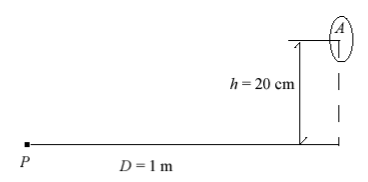
\includegraphics[width=0.6\linewidth]{HW1_Problem3.png}
\end{figure}
\bigbreak
\textbf{Solution}
\bigbreak
(a) From Slide 7 of Lecture 3 from NE806: Neutronics, the following equation is provided to determine the solid angle of the given geometry:
\bigbreak
\begin{equation*}
   \Omega  = 2\pi\bigg(1-\frac{D}{\sqrt{D^2+r^2}}\bigg)
\end{equation*}
\bigbreak
where $D$ is the distance between point $P$, and the disk. Based on the given parameters, the solid angle is found to be:
\bigbreak
\begin{equation*}
   \Omega  = 2\pi\bigg(1-\frac{100 cm}{\sqrt{(100 cm)^2+\frac{64cm^2}{\pi}}}\bigg) = \boxed{0.006390 \quad steradians}
\end{equation*}
\bigbreak


(b)
In order to avoid the difficulty incurred in the integral this problem would present, I utilized my knowledge from Monte Carlo class and solved this problem with MCNP6.
I used an isotropic point source at point P, then created a surface to tally over in the area of the circle shown in the figure.
All material was void, and the final flux result was simply multiplied by $4 \pi$ to obtain the solid angle.
One billion histories were used in the simulation.

$$ \boxed{\Omega \approx 6.14757 \times 10^{-3}}  $$
 
 
%%%%%%%%%%%%%%%%%%%%%%%%%%%%%%%%%%%%%%%%%%%%%%%%%%%%%%%%%%%%%%%%%%%%%%%%%%%%%%%%%%%%%%%%%%%%%%%%%%%%%%%%%%%%%%%%%
\newpage 
\textbf{Problem 4:} Consider the elastic scatter of a 1-MeV neutron with a nucleus of mass $ A=56$ for which the scatter angle in the COM frame is $\theta_c = 45^\circ$. \newline
(a) (5 points) What is the Q-value of the interaction? \newline
(b) (10 points) What is the scatter angle in the LAB frame? \newline
(c) (10 points) What is the energy of the scattered neutron? \newline
\textbf{Solution}
(a) From page 42 of Deuderstadt \& Hamilton, the following equation is given to determine the energy change of the neutron based on the atomic weight, $A$ of the target:
\bigbreak
\begin{equation*}
   E_f = \bigg[\frac{(1+\alpha)+(1-\alpha)cos(\theta_c)}{2}\bigg]E_i, \quad where \quad \alpha=\bigg(\frac{A-1}{A+1}\bigg)^2
\end{equation*}
\bigbreak
The Q value can be defined as the energy change of the neutron, $Q=E_i-E_f$, and $\alpha=.9311$ thus:
\bigbreak
\begin{equation*}
   Q = E_i\bigg(1- \bigg[\frac{(1.9311)+(0.0689)cos(45^\circ)}{2}\bigg]\bigg) \approx \boxed{0.0101 \quad MeV}
\end{equation*}
\bigbreak
(b) The scatter angle in the lab frame can be determine with an equation from page 41 of Deuderstadt \& Hamilton,
\bigbreak
\begin{equation*}
   \theta_L = tan^{-1}\bigg(\frac{sin(\theta_c)}{A^{-1}+cos(\theta_c)}\bigg) \approx \boxed{44.28^\circ}
\end{equation*}
\bigbreak
An interesting note about this result: the lab frame scatter angle and the COM frame scatter angle are very similar.
\bigbreak
(c) The energy of the neutron can be determined by taking the initial energy $E_i$ minus the Q-value:
\begin{equation*}
   E_f = 1 \quad MeV \quad - \quad 0.0101 \quad MeV \approx \boxed{0.9899 \quad MeV}
\end{equation*}
\end{document}
